\section{Metals}
\subsection{Properties of metals}

A metal is an element whose ion forms as a result of loss of electrons, i.e., elements whose ions
are positively charged are called metals. They exist between groups two to three in the Periodic
Table. 

In comparison to non-metals, metals are more thermally and electrically conductive. They are more
malleable, which means they can be beaten into many shapes. They are ductile as they can be wrought
out into wires. They tend to have high melting and boiling points.

The reactions of metals depend entirely on the metals themselves, or rather, the reactivity of 
the metals, which follow:
$$\underbrace{\ce {K} > \ce{Na} > \ce{Ca} > \ce{Mg} > \ce{Al}}_\text{high reactivity}>
\ce{C} > 
\underbrace{\ce{Zn} > \ce{Fe} > \ce{Pb}}_\text{moderate reactivity} > \ce{H} > 
\underbrace{\ce{Cu} > \ce{Ag} > \ce{Au}}_\text{low reactivity}
\footnote{where the metal to the
left of $>$ is more reactive than the ion to the right.
}$$
Note the
presence of the two non-metals: carbon and hydrogen. Though these are out of place, it is these
non-metals whose displacement or otherwise determined the reactivity of the metals. That is, the
metals more reactive than carbon are show high reactivity, those less reactive are moderate and
low reactive. Those that are more reactive than hydrogen show moderate and high reactivity, while
those are less reactive show low reactivity.

Metals with high and moderate reactivity react with dilute hydrochloric acid, displacing the
hydrogen in \ce{HCl} to give the corresponding metal chloride and hydrogen gas. So, lets consider
the reaction of a metal $\Lambda$ which is more reactive than hydrogen, with dilute hydrochloric
acid:
\begin{center}
\ce{2$\Lambda$(s) + 2HCl(aq) -> 2\Lambda Cl(aq) + H2(g)}
\end{center}
Note that, if $\Lambda$ is highly reactive, the above reaction is very strong and often infeasible.

Highly reactive metals, react with cold water directly, giving respective hydroxides and hydrogen.
An example with $\Lambda$ as the metal follows:
\begin{center}
	\ce{2$\Lambda$(s) + 2H2O(l) -> 2$\Lambda$OH(aq) + H2(g)}
\end{center}
Note that the ratio of OH to $\Lambda$ will depend on the electronic charges on the metal itself.

Moderately reactive metals react with water in the gaseous form, i.e., steam. The metal itself
must also be heated. 
Such a reaction always gives the metal oxide and hydrogen gas.
In this case, magnesium and aluminium act as moderately reactive metals. Once
again, with $\Lambda$ representing such a metal:
\begin{center}
	\ce{$\Lambda$(s) + H2O(g) -> $\Lambda$O(s) + H2(g)}
\end{center}

Metals with high and moderate reactivity both react with oxygen\footnote{Any reaction with oxygen
is called burning.}. The product is that metal's oxide:
\begin{center}
	\ce{2$\Lambda$(s) + O2(g) -> 2$\Lambda$O}
\end{center}
Note that, iron only reacts in the above reaction as powder or wool. 
Iron also reacts with air and moisture forming a layer of rust, which is hydrated iron(III) oxide.
Low reactive metals, such as
copper and lead react very slowly to give an oxide layer, under heat.

\subsection{Uses of metals}
Aluminium is a metal that shows low reactivity as a result of its oxide layer, which forms due
to its reaction with the air. It is a metal with very low density and hence is used in manufacturing
aircraft. It is also used in overhead electrical cables as it is a good electrical conductor and
low density. It is also used in food containers as it does not corrode easily as a result of the
oxide layer.

Copper is also a good electrical conductor, it is also ductile and is hence used in smaller scale
wiring.

\subsection{Alloys and their properties}
An alloy is a mixture of a metal with other elements. Brass is such a mixture consisting of copper
and zinc. Stainless steel is a mixture of iron and other elements such as chromium, nickel and
carbon.

The structure of a metal consists of layers of metal cations with a sea of delocalised electrons\footnote{
A delocalised electron is that which is not bound to any atom and can move freely}. These
layers are arranged such that they can cascade and slide over each other, which is why metals are
malleable and ductile. However, in alloys, the cations are differently sized due to the different
atoms present. This stops the layers from sliding easily, making alloys stronger and harder than
pure metals. A structure of a metal and an alloy follows:

\begin{center}
	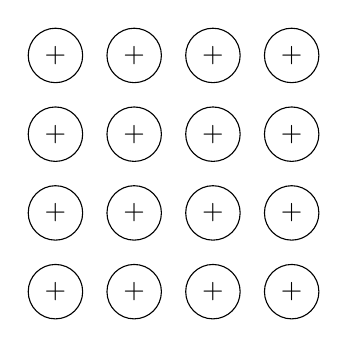
\begin{tikzpicture}
		\foreach \x in {1, 2, 3, 4}
			\foreach \y in {1, 2, 3, 4}
				\node[draw, circle] at (\x, \y) {$+$};
	\end{tikzpicture}

	A metal

	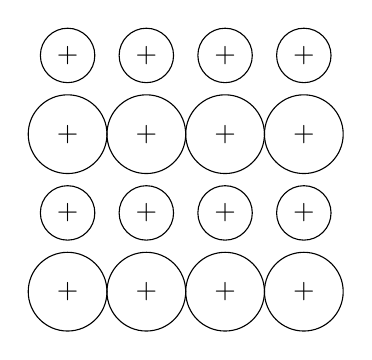
\begin{tikzpicture}
		\foreach \x in {1, 2, 3, 4} {
			\foreach \y in {1, 3}
				\node[draw, circle, minimum size=10mm] at (\x, \y) {$+$};
			\foreach \y in {2, 4}
				\node[draw, circle, minimum size=4mm] at (\x, \y) {$+$};
		};

	\end{tikzpicture}

	An alloy\footnote{These diagrams are far too bad to be acceptable answers to O-Level questions,
	please refer to prescribed book.}
\end{center}

\subsection{Reactivity series}
As shown at the beginning of the chapter, the order of reactivity of the metals is:
$$\underbrace{\ce {K} > \ce{Na} > \ce{Ca} > \ce{Mg} > \ce{Al}}_\text{high reactivity}>
\ce{C} > 
\underbrace{\ce{Zn} > \ce{Fe} > \ce{Pb}}_\text{moderate reactivity} > \ce{H} > 
\underbrace{\ce{Cu} > \ce{Ag} > \ce{Au}}_\text{low reactivity}
$$

The reactivity of a metal is said to be the tendency of the metal to form a positive ion. The 
relative reactivity of each metal is seen in displacement reactions involving the metals, where
the more reactive metal displaces the less reactive metal from its compound. An example follows,
where $\Lambda$ is a more reactive metal than $\Pi$.

\begin{center}
	\ce{$\Lambda$ + $\Pi$SO4 -> $\Pi$ + $\Lambda$SO4}
\end{center}
Note that, the less reactive metal is reduced and the more reactive metal is oxidised. The 
reactions of metals with water, hydrochloric acid and steam have all been discussed, some further
observations are given below.

Potassium, sodium and calcium have very strong reactions with cold water, where the potassium and
calcium are seen to skip over the water's surface while melting. Calcium reacts strongly. Magnesium,
only reacts with cold water very slowly, but burns with a brilliant flame when steam is passed over
heated magnesium.

Metals which are highly reactive have very violent reactions with dilute acid, so it is unsafe to
add them directly. 

Magnesium reacts strongly, disappearing into the acid while forming bubbles of
gas. The result is a colourless solution.

Aluminium is slow to react in cold acid, but bubbles form on heating, causing the aluminium to
disappear into the acid resulting in a colourless solution.

Zinc, disappears in cold acid, producing bubbles of gas and a colourless solution forms. Same is
the case with iron, only a pale green solution is formed.

Copper silver and gold, i.e., metals with low reactivity have no reaction with acids at all.

Aluminium, when kept exposed to air, reacts with the surrounding oxygen in the air resulting in
a layer of aluminium oxide around the sample of aluminium. This layer is unreactive, so aluminium
is \textit{apparently} unreactive as the layer is non porous and no oxygen can reach the 
underlying aluminium.

Given a set of experimental observations, using the strength of reactions described and the 
knowledge from the reactivity series of metals, we can deduce the reactivity of given metals.

\subsection{Corrosion of metals}
Metals corrode under certain conditions as results of certain reactions.

Iron and steel corrode in presence of oxygen or water producing a layer of iron (III) oxide, called
rust. Prevention of this comes down to many strategies, including barrier protection, where the
metal is either coated by another or painted so as to prevent contact of water and oxygen with the
metal. Barriers used to protect metals from corrosion can be painting, greasing or coating the
metal with plastic.

Sacrificial protection consists of another more reactive metal being placed adjacent the metal
to be protected. The moisture and air will then react with the more reactive metal in precedence to
the relatively less reactive metal. In other words, the higher reactive metal loses electrons more
readily, as a result, that metal is oxidised and the lower reactive metal is not corroded.

The two strategies can be combined in that zinc can be used to electroplate any metal, where since
zinc is more reactive, it will be reduced in precedence to the metal being coated. The disadvantage
to barrier protection is that when the coating comes off, that area will immediately be corroded.
This method prevents that as even if the layer is scratched, the moisture will react with the zinc
instead. This method is called galvanising.

\subsection{Extraction of metals}
Metals can be extracted easily depending on their reactivity.

Iron is found naturally in an ore called haematite, which is iron (III) oxide. Iron is extracted
from iron (III) oxide in a blast furnace, by means of reduction by carbon monoxide.

Raw materials, iron ore, coke (carbon made from coal) and the mineral\footnote{A naturally ocurring
rock containing a particular compound} limestone. The furnace has blasts of hot air sent near
the bottom, allowing a series of chemical reactions to occur resulting in the production of pure
iron.

Firstly, the coke burns in the air blast and the furnace gets very hot from this exothermic
reaction:
$$ \ce{C + O2 -> CO2} $$
As carbon dioxide rises through the furnace it reacts with more carbon and is reduced to carbon
monoxide:
$$ \ce{CO2 + C -> 2CO} $$
The most important reaction is the reduction of haematite by this carbon monoxide
$$ \ce{Fe2O3 + 2CO -> 2Fe + CO2} $$
This produced iron flows to the bottom of the furnace where it can be tapped off.

Iron ore contains the impurity sand, which is silicon (IV) oxide, also called silica. Limestone,
calcium carbonate
is added to the blast furnace to rid the iron of this impurity. Firstly, the calcium carbonate
decomposes in the heat of the furnace:
$$ \ce{CaCO3 -> CaO + CO2} $$
Subsequently, this calcium oxide reacts with silica to form calcium silicate, also called slag.
$$ \ce{SiO2 + CaO -> CaSiO3} $$

Aluminium is a metal that shows high reactivity, as a result reduction cannot be used for its 
extraction, rather, electrolysis is employed.

Cryolite is used as a solvent for aluminium as it reduces the melting point of the substance 
allowing the mixture to be liquid at lower temperatures which is economical. It also conducts
electricity and as a result can be used in electrolysis.

The ore for aluminium is bauxite, which is simply aluminium oxide.

Bauxite, dissolved in cryolite is electrolysed using carbon electrodes. The cathode reactions
are as follows:
\begin{center}
	at cathode: \ce{Al^{3+}(l) + 3e- -> Al(l)}

	at anode: \ce{2O^{2-}(l) -> O2(g) + 4e-}
\end{center}

At the very high temperature of the electrolysis conditions, the oxygen being formed at the anode
burns the carbon in the anode,
$$\ce{C(s) + O2(g) -> CO2(g)}$$
forming carbon dioxide and causing the anodes to corrode and be regularly replaced.
